\section{Gefahrenanalyse}
% Gesellschaftliche Betrachtung der Thematik.
% 2-3 Sätze die erklären, was im Kapitel passiert.
In diesem Kapitel werden die Angriffspunkte von Deepfakes und den damit verbundenen Gefahren für die Gesellschaft beschrieben.
Anhand einiger Beispiele wird aufgezeigt, welchen Einfluss Deepfakes haben, um beim Menschen durch gezielte Manipulation Schaden anzurichten.
Weiterhin werden Möglichkeiten zur schnelleren Erkennung solcher Manipulationen diskutiert.
\subsection{Gefahrenpotential allgemein}\label{Gefahrenpotential}
% Hier zunächst allgemeine Gefahrenpotentiale von gezielter Fehlinformation definieren.
Das Konzept der Falschinformation, in der heutigen Zeit oft unter dem Begriff ``Fake News'' genannt, ist eine Methode die bereits seit mehr als 125 Jahren eingesetzt wird um Menschen gezielt zu manipulieren.
Gerade im Zeitalter der sozialen Medien, in denen sich Menschen öfter dieser Meldungen bedienen als konventioneller Nachrichten, wächst die Bedrohung durch Falschinformation täglich (\cite{Lee2019}).
Eine große Gefahr die dabei von Deepfakes ausgeht, ist dass jeder die Möglichkeit hat, diese mit kostenfreier Software zu erstellen (\cite{Appel2022}).
Das gefährliche dabei ist die millionenfache Verbreitung innerhalb Sekunden um die ganze Welt, in der Jeder Ziel eines solchen Angriffs sein kann (\cite{Shahzad2022}).
\par
Dabei nennen Appel und Prietzl (\cite{Appel2022}) Angriffsziele von privaten Personen, über Prominente Personen bis hin zu ganzen Staaten.
Besonders letzteres ist ein immer häufiger gewähltes Ziel, gerade bei politschen Wahlen oder Zwischenstaatlichen Beziehungen.
So kursierte im März 2022 in sozialen Medien ein Deepfake-Video des Ukrainischen Präsidenten Volodymyr Zelenskyy, in dem er im Rahmen des Russisch-ukrainischen Krieges die Kapitulation seiner Soldaten forderte.
Einmal durch die Kanäle sozialer Medien verbreitet, lassen sich diese Falschmeldungen schwierig Löschen oder Richtigstellen und wenn doch, dann ist der Schaden bereits angerichtet.
Soziale Netzwerke oder Messenger wie Facebook, WhatsApp oder Telegram sind dabei besonders kritisch zu betrachten, da sie die Verbreitung von ungeprüften Inhalten jeglicher Art ermöglichen (Vgl. \cite{Appel2022}).
\par
Deepfakes erweitern und verschlimmern also das bereits bekannte Phänomen der ``Fake News'', indem sie sich der gleichen Kanäle bedienen, die Inhalte allerdings noch deutlich realistischer und glaubhafter darstellen (\cite{Appel2022}).
Gerade das hohe Level von Faktoren wie Verbreitungsgeschwindigkeit, Realismus und Personalisierung machen Deepfakes zu einer immer weiter wachsenden Gefahr für die Gesellschaft.
Was den Menschen dabei so angreifbar macht, ist die Tatsache, dass vermeintlich selbst wahrgenommen Inhalte wie Videos und Fotos, einen stärkeren Eindruck hinterlassen als niedergschriebener Text.
Besonders wenn es sich dabei um vertraute Personen und deren Auftreten oder Stimme handelt (\cite{Kietzmann2020})
\newpage

\subsection{Gefahrenanalyse am Beispiel aktueller Fälle}\label{GefahrenAktuelleFaelle}
% Gefahrenpotentiale an Beispielen konkretisieren: \textbf{Was} wurde gemacht um \textbf{was} zu erreichen?
% Hier Fokus auf Echtzeitproblematik legen? Oder folgt das aus dem nächsten Unterkapitel?
Folgend werden einige aus dem unter Abschnitt \ref{Gefahrenpotential} beschriebenen Gefahren anhand konkreter Realfällen diskutiert.
Bei diesen Fällen handelt es sich hauptsächlich um Betrugsfälle, die mit Hilfe von Deepfakes durchgeführt wurden.
\par
Einer dieser Fälle, der im Zusammenhang mit Deepfake-Betrug genannt wird, ist die Erbeutung von 220.000\euro{} durch Verwendung eines Audio-Deepfakes.
In diesem Fall stellten Betrüger die Stimme eines CEO am Telefon nach und baten seinen angeblichen Mitarbeiter, den genannten Betrag auf ein Konto zu überweisen (CITE ONLINE QUELLE?!).
Der angerufene Mann berichtete nachträglich an die Ermittlungsbeamten, dass er den deutschen Akzent und die Melodie der Stimme seines CEO's erkannte, und somit keinen Verdacht schöpfte dass es sich bei diesem Anrufer um einen Betrüger handelte.
Die Ermittlungen gingen davon aus, dass eine kommerzielle Software zur Erstellung des Deepfakes verwendet wurde.
Dieses Beispiel verdeutlicht, dass jeder mit entsprechender freizugänglicher Software im Stande ist, so einen Betrug mit Hilfe eines Audio-Deepfakes durchzuführen. (CITE ONLINE QUELLE?!).
\par
Eine weitere Betrugsmasche, vor der das FBI offiziell warnte, sind Betrugsfälle in denen sich mit durch Video Deepfake veränderter Stimme für sensible Jobs beworben wird.
Während dieser Jobinterviews, die meist auf Jobs mit Heimarbeit in Softwareunternehmen mit großen Datenmengen abzielen, benutzen Betrüger die Stimme einer anderen Person.
Das FBI betonte hierbei aber, dass die Synchronisation zwischen Lippenbewegung und Sprache nicht komplett übereinstimmte.
Somit gibt es Anhaltspunkte zur Vorbeugung und Erkennung solcher Betrüge in Form von Jobinterviews, indem Mitarbeiter von Unternehmen geschult werden um unter anderem auf solche Merkmale verschärft zu achten (CITE QUELLE FBI).
\par
Zur Veranschaulichung der potentiellen politschen Manipulation unter der Verwendung von Deepfakes, ist die Rede der amerikanischen Politikerin Nancy Pelosi aus dem Jahr 2019 zu nennen (ZITIER https://perma.cc/A26H-4PF3?type=image).
In dieser Rede wurde das Videomaterial so manipuliert, dass es so scheint als ob sie stotterte und undeutlich rede.
Das manipulierte Video wurde von dem zu dieser Zeit amerikanischen Staatspräsidenten und Anhänger der Gegnerpartei von Nancy Pelosi, Donald Trump, über Twitter verbreitet.
Er teilte es mit den Worten ``Pelosi stammers through news conference'', also mit der gezielten Absicht sie mit Hilfe dieses Videos zu diffamieren (ZITIER https://perma.cc/A26H-4PF3?type=image).
\par
Dieses Video zeigt die Gefahr der schnellen Verbreitung von ungeprüften Inhalten durch soziale Medien, die unter Abschnitt \ref{Gefahrenpotential} genannt wurde.
Über Facebook wurde dieses Video über 2.5 Millionen mal angeschaut, Facebook selbst lies dieses Video auf der Plattform bestehen versprach aber die Verbreitung einzugrenzen.
Youtube hingegen löschte dieses Video, da es sich um falsche Inhalte handelte.
Dieses unterschiedliche Behandeln von Falschinformation verschiedener sozialer Medien zeigt die Schwierigkeit des Konsums von Informationen über diese Plattformen.
Es bleibt daher ein beliebtes Mittel zur Verbreitung solcher Inhalte, eben aufgrund der freien Verbreitung, Geschwindigkeit und umständlicher Löschung dieser (\cite{Appel2022}).
\par
Die hier beschriebenen Betrugsfälle veranschaulichen, dass wie unter Abschnitt \ref{Gefahrenpotential} beschrieben, mit einfachsten Mitteln großer Schaden angerichtet werden kann.
Besonders die von Kietzmann (\cite{Kietzmann2020}) beschriebene Vertrautheit von Inhalten wie z.B. die Stimme im Zusammenspiel mit Gestik und Mimik, ließ bei den erwähnten Beispielen keinen Zweifel an der Echtheit.
So reichte es bei dem Telefonbetrug, dass der deutsche Akzent und die Melodie der Stimme vermeintlich übereinstimmte, keinen Verdacht zu schöpfen.
Darüberhinaus zeigen die genannten Beispiele, dass die Echtzeit und damit die nahezu nicht vorhandene Zeit zur Erkennung eine entscheidene Rolle spielt.
Einmal verbreitet lässt sich der Schaden nur erschwert beheben oder die Inhalte schwierig Löschen oder Richtigstellen (\cite{Shahzad2022}).
Dabei betonte Shahzad (\cite{Shahzad2022}) einmal mehr, zukünftig effektive Methoden zur Erkennung in Echtzeit zu entwickeln, da diese den Großteil der Bedrohung darstellen.
Ein weiteres Gefahrenpotential bleibt der einfache Zugang zur Erstellung solcher Deepfakes.
Mit den richtigen Zugängen zu Verbreitungskanälen und anzusprechenden Opfern, ist es jedem Menschen möglich das Mittel der Manipulation durch Deepfakes zum Betrug einzusetzen (\cite{Appel2022}).




\subsection{Gefahrenanalyse/Studien zur menschlichen Wahrnehmung}
% Analyse von durchgeführten Studien: Inwieweit ist der Mensch anfällig für Deepfakes?
% Welche Konsequenz ergibt sich daraus? (Anforderungen an Informationen, Detektion von DF, etc.)
Folgend werden Ergebnisse mehrerer Studien betrachtet, um den Einfluss und die damit verbundenen Gefahren von Deepfakes auf den Menschen zu betrachten.
Die menschliche Wahrnehmung von Deepfakes sowie Folgen der Manipulation spielen sind dabei Hauptfaktoren.
\par
Um zu untersuchen, ob und mit welchem Umfang Deepfakes im politschen Rahmen Wähler beeinflussbar sind, manipulierten Wissenschaftler der Amsterdamer Universität Videomaterial eines holländischen Politikers \citep[Vgl.][]{Dobber2020}.
In diesem dreizehn sekündigen Video beinhalten die letzten fünf Sekunden manipuliertes Material in dem der folgene Satz fällt ``But, as Christ would say: don’t crucify me for it''.
Sie wählten diesen Satz, da dieser Politker einer konservativen christlichen Partei angehörte und somit die potentielle Wahlzielgruppe anspricht.
Dabei nutzte diese Studie politisches Microtargeting, ein von Parteien zur Beeinflussung von Wählern häufig gewähltes Mittel, indem es auf die religiöse Einstellung abzielte \citep[Vgl.][]{Papakyriakopoulos2017}.
\par
An dieser Studie nahmen 277 Menschen teil, von denen 144 Teilnehmer das manipulierte Video und 133 das Originalvideo sahen.
Schlüsselfaktoren zur Einteilung und Unterscheidung waren unter anderem die Religiösität und die politische Einstellung.
Als Ergebnis betrachtete die Studie die Einstellung der Teilnehmer gegenüber dem Politker und seiner Partei.
Gläubige Menschen, die das manipulierte Videon sahen, hatten eine schlechtere Einstellung zum Politker als vorher.
Dabei galt diese schlechtere Einstellung eher dem Politiker direkt, als seiner angehörigen Partei.
Von den 144 Teilnehmern, die das manipulierte Video sahen, erkannten nur 12 den Fake.
Zukünftige Erstellung von realistischeren Deepfakes könnte dies aber ändern, Potential zur Manipulation durch Deepfakes sei gegeben.
Durch die Verwendung von Deepfakes lassen sich Menschen leichter manipulieren als durch klassische ``Fake News'' \citep[][]{Dobber2020}.
Weiterhin kam die Studie zum Fazit, dass sich aufgrund der geringen Anzahl von 12 Leuten die den Fake erkannten, die Sensibiliserung der Gesellschaft für solche Deppfakes verbessern sollte.
Diese Studie zeigt die Gefahr der Fähigkeit, eine bestimmte politische oder demographische Gruppe anzusprechen.
Es kann also gezielt Microtargetting über soziale Medien betrieben werden \citep[Vgl.][]{Hancock2021}.
\newpage
Zur Analyse, ob und wie der Mensch manipulierte Audiodateien erkennt, erschufen sie ein rundenbasiertes Spiel \citep[][]{Mueller2022}.
In Jeder Runde, hörten die Teilnehmer eine Audio und mussten wählen ob diese echt oder gefaked ist.
Dazu hörten die 410 Teilnehmer insgesamt 13229 Audiodateien, wobei nur gezählt wurde wenn mindestens 10 Runden absolviert waren.
\par
\begin{figure}[h]
 \centering
 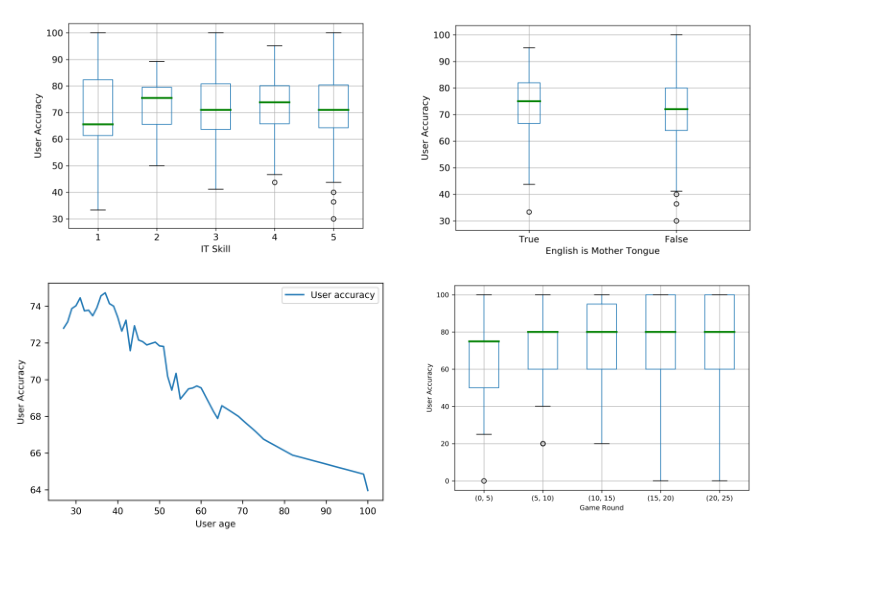
\includegraphics[width=\textwidth]{Assets/ResultsHumanDetectionDeepFake.png}
 \caption{Menschliche Wahrnehmung von Audio Deepfakes \citep[][]{Mueller2022}.}
 \label{fig:ResultsDetectionDeepfake}
\end{figure}
Die Teilnehmer wurden an Faktoren wie Alter, IT-Erfahrungen und Muttersprachler (die Studie wurde in englischer Sprache durchgeführt) kategorisiert.
Unter Abbildung \ref{fig:ResultsDetectionDeepfake} sind die Ergebnisse zu erkennen, in denen die Genauigkeit der Erkennung dem jeweiligen Personenkreis gegenüber gestellt ist.
Muttersprachler haben Vorteile bei der Erkennung von Fakes gegenüber Fremdsprachlern.
Weiterhin sei die IT-Kenntniss irrelevant, mit zunehmendem Alter verschlechterte sich die Genauigkeit. 
In den Ersten Runden nimmt die Genauigkeit bei der Erkennung zu, stagniert dann aber nach etwa 20 Runden.
Schaffung der Förderung von zukünftigen Gegenmaßnahmen werden benötigt, da sich die Qualität der Audio-Deepfakes erhöht, die menschlichen Fähigkeiten zur Erkennung allerdings stagnieren \citep[][]{Mueller2022}.
\par
Zur Untersuchung, welchen sozialen Einfluss Deepfakes auf den Menschen haben, verbindet Hancock das Verhalten des Menschen auf generelle Falschinformationen mit der Täuschung von Deepfakes.
Menschen sind, so Hancock, nicht gut darin Falschinformationen als solche zu erkennen.
Es wird dazu geneigt, eher an das zu Glauben was gesehen wird.
Das gefährliche an Deepfakes ist die manipulierte Kombination von z.B. Stimme, Mimik und Gestik.
Während einer dieser Faktoren schon schwierig als Falschinformation zu entlarven ist, verstärkt diese Kombination durch Vertrautheit der Wahrnehmung die Glaubhaftigkeit des Fakes \citep[Vgl.][]{Hancock2021}.
Durch Sensibilisierung lassen sich die Effekte schmälern, so vergleich Hancock es mit der Existenz von Spammails, deren Gefahr durch allgemeine Bekanntheit innerhalb der Gesellschaft verringert ist.







% Analyse von durchgeführten Studien: Inwieweit ist der Mensch anfällig für Deepfakes?
% Welche Konsequenz ergibt sich daraus? (Anforderungen an Informationen, Detektion von DF, etc.)